%----------------------------------------------------------------------------
\chapter{Mérési feladatok}\label{sect:LatexTools}
%----------------------------------------------------------------------------
%
%\begin{figure}[!ht]
%	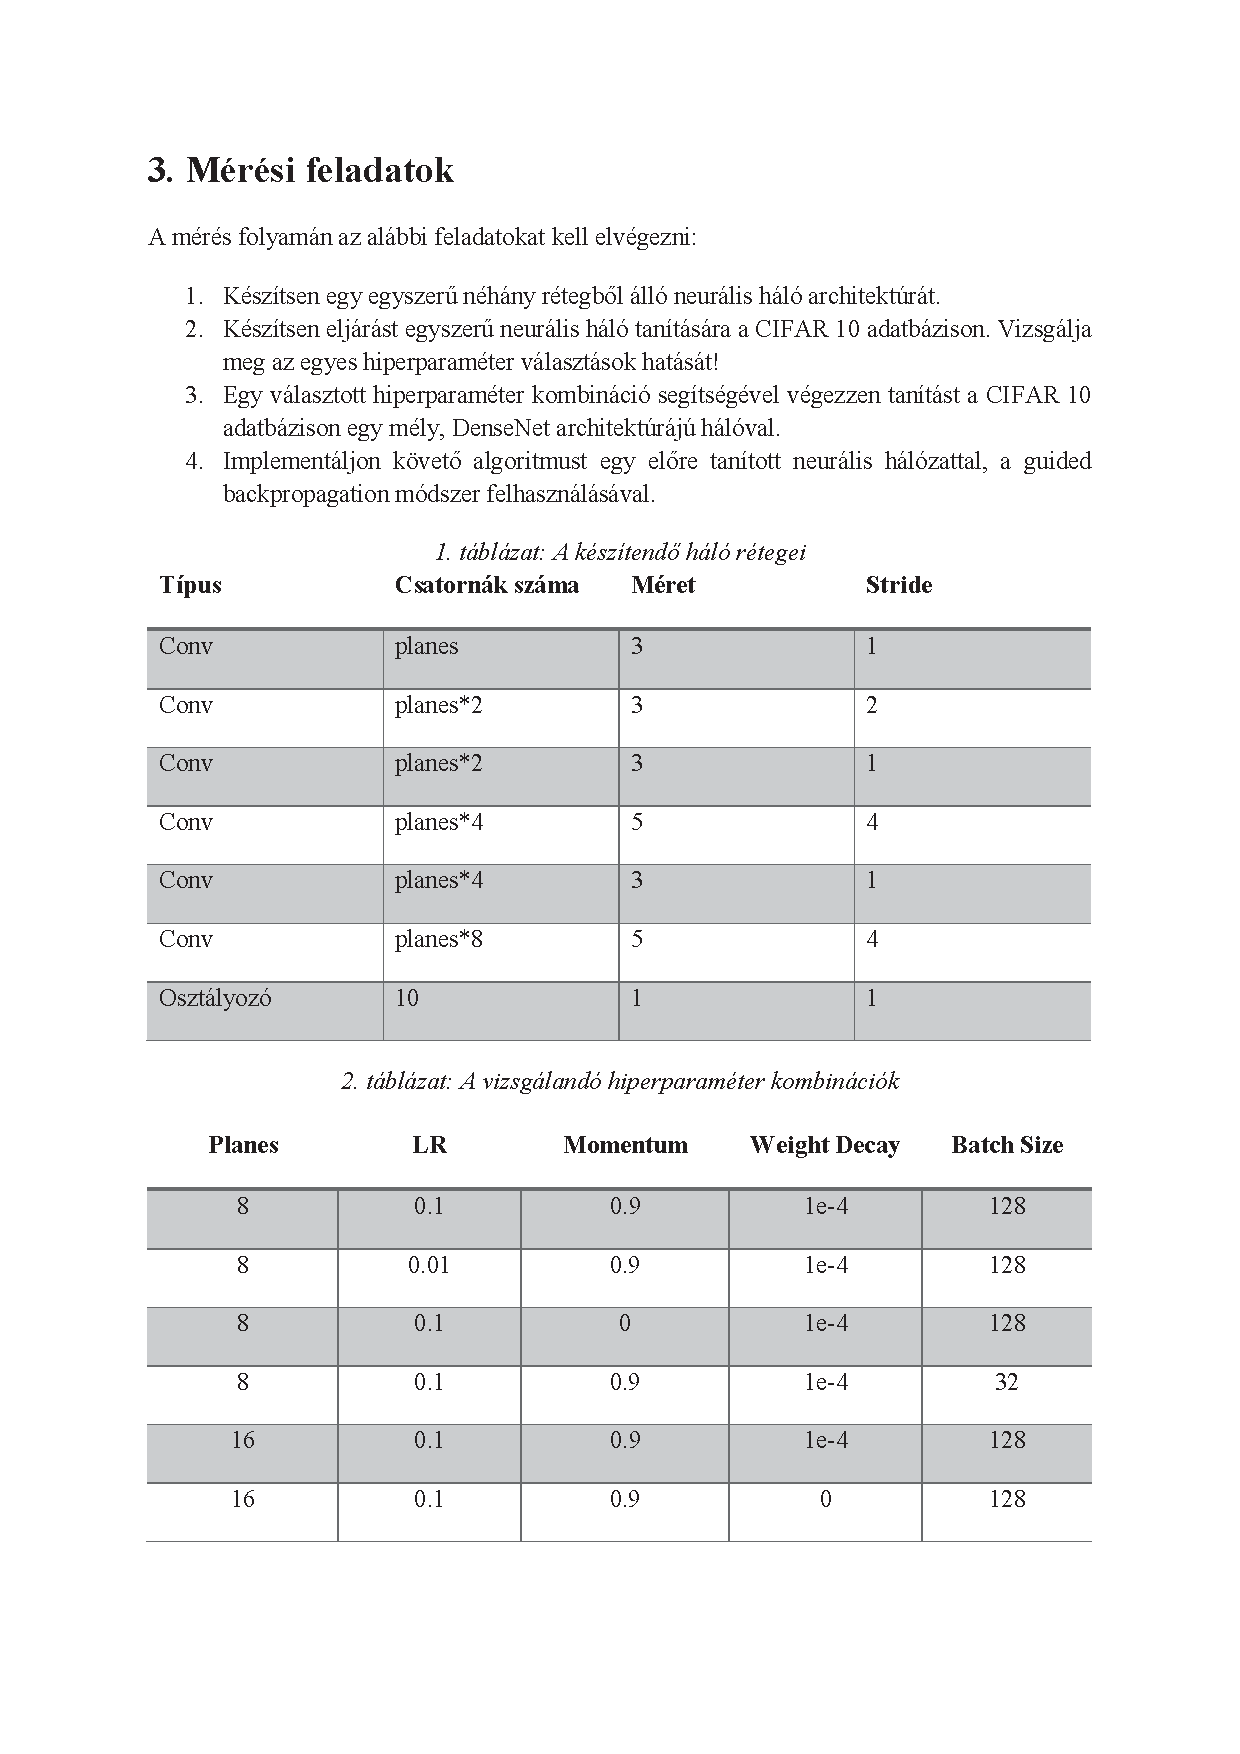
\includegraphics[trim = 25mm 210mm 20mm 33mm,clip, width=150mm,keepaspectratio]{figures/feladatok_m07.pdf}
%	\label{fig:Road-of-a-char}
%\end{figure}

A mérés folyamán az alábbi feladatokat kell elvégezni:
\begin{enumerate}
	\item Alkossa meg a sorompó, az infrakapu és a távirányító modelljét! Ügyeljen az események irányíthatóságának helyes megválasztására!
	\item Fogalmazza meg azon specifikációkat, amelyeknek a zárt rendszer működés során eleget kell, hogy tegyen! Alkossa meg ezen specifikációk modelljét!
	\item A Supremica program segítségével tervezze meg azt a felügyeleti szabályozót, amellyel biztosítani tudja az előzőekben meghatározott specifikációk betartását!
	\item Implementálja és tesztelje a szabályozót Stateflow-környezetben!
\end{enumerate}
